\documentclass[11pt]{article}

%%%%%%%%%%%%%%%%%%%%%%%%%%%%%%%%%%%%%%%%%%%%%%%%%%%%%%%%%%%%%%%%%%%%%%
%\pdfminorversion=4
% NOTE: To produce blinded version, replace "0" with "1" below.
\newcommand{\blind}{0}

%%%%%%% IISE Transactions margin specifications %%%%%%%%%%%%%%%%%%%
\addtolength{\oddsidemargin}{-.5in}%
\addtolength{\evensidemargin}{-.5in}%
\addtolength{\textwidth}{1in}%
\addtolength{\textheight}{1.3in}%
\addtolength{\topmargin}{-.8in}%

\makeatletter
\renewcommand\section{\@startsection {section}{1}{\z@}%
	{-3.5ex \@plus -1ex \@minus -.2ex}%
	{2.3ex \@plus.2ex}%
	{\normalfont\fontfamily{phv}\fontsize{16}{19}\bfseries}}
\renewcommand\subsection{\@startsection{subsection}{2}{\z@}%
	{-3.25ex\@plus -1ex \@minus -.2ex}%
	{1.5ex \@plus .2ex}%
	{\normalfont\fontfamily{phv}\fontsize{14}{17}\bfseries}}
\renewcommand\subsubsection{\@startsection{subsubsection}{3}{\z@}%
	{-3.25ex\@plus -1ex \@minus -.2ex}%
	{1.5ex \@plus .2ex}%
	{\normalfont\normalsize\fontfamily{phv}\fontsize{14}{17}\selectfont}}
\makeatother
%%%%%%%%%%%%%%%%%%%%%%%%%%%%%%%%%%%%%%%%%%%%%%%%%%%%%%%%%%%%%%%%%%%%%%%%%

%%%%% IISE Transactions package list %%%%%%%%%%%%%%%%%%%%%%%%%%%%%%%%%%%%%%
\usepackage{amsmath}
\usepackage{graphicx}
\usepackage{enumerate}
\usepackage{natbib} 
\usepackage{url} 
\usepackage{xcolor}
\usepackage{enumitem}
\usepackage{amssymb}
\usepackage{algorithm}
\usepackage{algpseudocode}
\usepackage{bm}
\usepackage{setspace}
\usepackage{float} 
\usepackage{subcaption}
\usepackage{booktabs} 
\usepackage{multirow} 

\begin{document}
	
	%%%%%%%%%%%%%%%%%%%%%%%%%%%%%%%%%%%%%%%%%%%%%%%%%%%%%%%%%%%%%%%%%%%%%%%%%%%%%%
	\def\spacingset#1{\renewcommand{\baselinestretch}%
		{#1}\small\normalsize} \spacingset{1}
	%%%%%%%%%%%%%%%%%%%%%%%%%%%%%%%%%%%%%%%%%%%%%%%%%%%%%%%%%%%%%%%%%%%%%%%%%%%%%%
	
	% =========================================================================
	%                           单独文件的标题页设置
	% =========================================================================
	
	\if0\blind
	{
		\begin{center}
			% 标题：明确指出是补充材料
			{\LARGE \bfseries Supplementary Materials for: \\[\baselineskip]
				``Dual-Attention Deep Gaussian Processes for Multi-Objective Robust Parameter Design''} 
			
			\vspace{0.8cm} % 间距
			
			% 作者信息
			
		\end{center}
	} \fi
	
	\if1\blind
	{
		\bigskip
		\begin{center}
			{\LARGE \bfseries Supplementary Materials for: \\[\baselineskip]
				``Dual-Attention Deep Gaussian Processes for Multi-Objective Robust Parameter Design''}
		\end{center}
		\medskip
	} \fi
	
	\bigskip
	\bigskip
	
	% =========================================================================
	%                           附录内容设置
	% =========================================================================
	
	\appendix % 将后续 Section 编号改为 A, B, C...
	
	% --- 设置公式、图表的编号格式为 A.1, B.1 等 ---
	\renewcommand{\theequation}{\Alph{section}.\arabic{equation}}
	\renewcommand{\thefigure}{\Alph{section}.\arabic{figure}}
	\renewcommand{\thetable}{\Alph{section}.\arabic{table}}
	\setcounter{equation}{0}
	\setcounter{figure}{0}
	\setcounter{table}{0}
	
	% ---------------- Appendix A ----------------
	% 您可以在这里修改标题，例如 "Proofs" 或 "Mathematical Derivations"
	\section{Derivation of the Variational ELBO for Sparse GPs} \label{app:A}
	\setcounter{equation}{0} % 确保这一节的公式从 A.1 开始
	
	This appendix provides a detailed derivation of the Evidence Lower Bound (ELBO) (Equation 4) described in Section 2.2. We consider the augmented GP model by introducing $M$ inducing points $\mathbf{Z}$ and corresponding inducing variables $\mathbf{u}$. The joint probability of the observations $\mathbf{y}$, latent functions $\mathbf{f}$, and inducing variables $\mathbf{u}$ is given by:
	\begin{equation}
		p({\bf{y}},{\bf{f}},{\bf{u}}) = p({\bf{y}}|{\bf{f}})p({\bf{f}}|{\bf{u}})p({\bf{u}}),
	\end{equation}
	where $p(\mathbf{u}) = \mathcal{N}(\mathbf{0}, \mathbf{K}_{\mathbf{uu}})$ is the prior over inducing variables, and $p(\mathbf{f} | \mathbf{u})$ follows the standard GP conditional distribution. To approximate the intractable posterior $p(\mathbf{f}, \mathbf{u} | \mathbf{y})$, we propose a variational distribution $q(\mathbf{f}, \mathbf{u})$. Following the framework of Titsias (2009), we enforce the variational posterior to factorize as:
	\begin{equation}
		q({\bf{f}},{\bf{u}}) = p({\bf{f}}|{\bf{u}})q({\bf{u}}),
	\end{equation}
	where $q(\mathbf{u}) = \mathcal{N}(\mathbf{m}, \mathbf{S})$ is a free variational distribution to be optimized, and $p(\mathbf{f} | \mathbf{u})$ is fixed to the model prior conditionals. This corresponds to Equation (4) in the main text.The goal of variational inference is to minimize the Kullback-Leibler (KL) divergence between the approximate posterior and the true posterior, which is equivalent to maximizing the ELBO:
	\begin{equation}
		\mathcal{L} = \iint q(\mathbf{f}, \mathbf{u}) \log \frac{p(\mathbf{y}, \mathbf{f}, \mathbf{u})}{q(\mathbf{f}, \mathbf{u})} \, d\mathbf{f} d\mathbf{u}
	\end{equation}
	
	Substituting (A.1) and (A.2) into (A.3), the ELBO can be expanded as:
	\begin{equation}
		\begin{aligned}
			\mathcal{L} &= \iint p(\mathbf{f}|\mathbf{u})q(\mathbf{u}) \log \frac{p(\mathbf{y}|\mathbf{f})p(\mathbf{f}|\mathbf{u})p(\mathbf{u})}{p(\mathbf{f}|\mathbf{u})q(\mathbf{u})} \, d\mathbf{f}d\mathbf{u} \\
			&= \iint p(\mathbf{f}|\mathbf{u})q(\mathbf{u}) \left[ \log p(\mathbf{y}|\mathbf{f}) + \log \frac{p(\mathbf{u})}{q(\mathbf{u})} \right] \, d\mathbf{f}d\mathbf{u}
		\end{aligned}.
	\end{equation}
	
	The term $p(\mathbf{f} | \mathbf{u})$ cancels out in the logarithm ratio, significantly simplifying the computation. The equation splits into two components:
	
	(1) Expected Log-Likelihood:
	\begin{equation}
		\iint q(\mathbf{u})\,p(\mathbf{f}\mid \mathbf{u})\,\log p(\mathbf{y}\mid \mathbf{f})\,d\mathbf{f}\,d\mathbf{u}
		= \mathbb{E}_{q(\mathbf{f})}\!\left[\log p(\mathbf{y}\mid \mathbf{f})\right]
		= \sum_{i=1}^{N}\mathbb{E}_{q(f_i)}\!\left[\log p(y_i\mid f_i)\right],
	\end{equation}
	where $q(\mathbf{f}) = \int p(\mathbf{f} | \mathbf{u}) q(\mathbf{u}) d\mathbf{u}$ represents the marginal variational distribution.
	
	(2) KL Divergence:
	\begin{equation}
		\int q(\mathbf{u})\left[\int p(\mathbf{f}\mid \mathbf{u})\,d\mathbf{f}\right]
		\log\frac{p(\mathbf{u})}{q(\mathbf{u})}\,d\mathbf{u}
		= -\mathrm{KL}\!\left[q(\mathbf{u})\,\|\,p(\mathbf{u})\right].
	\end{equation}
	Note that $\int p(\mathbf{f} | \mathbf{u}) d\mathbf{f} = 1$.
	Combining (A.5) and (A.6), we obtain the final ELBO formulation as presented in Equation (4):
	\begin{equation}
		\mathcal{L}_{\mathrm{SGP}}
		= \sum_{i=1}^{N}\mathbb{E}_{q(f_i)}\!\left[\log p(y_i\mid f_i)\right]
		- \mathrm{KL}\!\left[q(\mathbf{u})\,\|\,p(\mathbf{u})\right].
	\end{equation}
	
	
	
	
	
	
	
	
	
	
	% ---------------- Appendix B ----------------
	% 您可以在这里修改标题，例如 "Additional Experiments"
	\section{Proof of Unbiased Gradient Estimation via Reparameterization Trick} \label{app:B}
	\setcounter{equation}{0}
	
	This appendix provides the mathematical justification for the gradient computation in the Doubly Stochastic Variational Inference (DSVI) framework, specifically concerning Equations (9)-(12) in Section 2.3.
	We aim to compute the gradient of the expected log-likelihood term in the ELBO with respect to the variational parameters $\boldsymbol{\phi}$ (i.e., $\mathbf{m}, \mathbf{S}$). The objective function is:
	\begin{equation}
		\mathcal{L}(\phi)
		= \mathbb{E}_{q_{\phi}(\mathbf{f})}\!\left[\log p(\mathbf{y}\mid \mathbf{f})\right]
		= \int q_{\phi}(\mathbf{f})\,\log p(\mathbf{y}\mid \mathbf{f})\,d\mathbf{f}.
	\end{equation}
	Directly differentiating (B.1) is problematic because the integration domain depends on $\boldsymbol{\phi}$. To resolve this, we apply the reparameterization trick defined in Equation (11):
	\begin{equation}
		\mathbf{f}
		= g(\phi,\boldsymbol{\epsilon})
		= \boldsymbol{\mu}_{\phi} + \boldsymbol{\Sigma}_{\phi}^{1/2}\odot \boldsymbol{\epsilon},
		\qquad
		\boldsymbol{\epsilon}\sim p(\boldsymbol{\epsilon})=\mathcal{N}(\mathbf{0},\mathbf{I}).
	\end{equation}
	Using the Law of the Unconscious Statistician (LOTUS), the expectation over $q_{\boldsymbol{\phi}}(\mathbf{f})$ can be rewritten as an expectation over the auxiliary noise distribution $p(\boldsymbol{\epsilon})$, which is independent of $\boldsymbol{\phi}$:
	\begin{equation}
		\mathcal{L}(\phi)
		= \mathbb{E}_{p(\boldsymbol{\epsilon})}\!\left[\log p\!\left(\mathbf{y}\mid g(\phi,\boldsymbol{\epsilon})\right)\right].
	\end{equation}
	Now, the gradient operator $\nabla_{\boldsymbol{\phi}}$ can be moved inside the expectation:
	\begin{equation}
		\nabla_{\phi}\mathcal{L}(\phi)
		= \nabla_{\phi}\int p(\boldsymbol{\epsilon})\,\log p\!\left(\mathbf{y}\mid g(\phi,\boldsymbol{\epsilon})\right)\,d\boldsymbol{\epsilon}
		= \mathbb{E}_{p(\boldsymbol{\epsilon})}\!\left[\nabla_{\phi}\log p\!\left(\mathbf{y}\mid g(\phi,\boldsymbol{\epsilon})\right)\right].
	\end{equation}
	This expectation can be efficiently approximated using Monte Carlo sampling. For $S$ samples of $\boldsymbol{\epsilon}_s \sim \mathcal{N}(\mathbf{0}, \mathbf{I})$:
	\begin{equation}
		\nabla_{\phi}\mathcal{L}(\phi)
		\approx \frac{1}{S}\sum_{s=1}^{S}\nabla_{\phi}\log p\!\left(\mathbf{y}\mid g(\phi,\boldsymbol{\epsilon}_s)\right).
	\end{equation}
	Since $g(\boldsymbol{\phi}, \boldsymbol{\epsilon})$ is a deterministic differentiable function, the gradients can be computed via standard backpropagation (chain rule). This proves that the reparameterization trick provides an unbiased low-variance gradient estimator for optimizing the ELBO in Equation (9).
	
	
	% ---------------- Appendix C ----------------
	% 您可以在这里修改标题，例如 "Sensitivity Analysis"
	\section{Theoretical Justification of the Weighted ELBO} \label{app:C}
	\setcounter{equation}{0}
	
	This appendix provides the theoretical basis for the sample-weighted ELBO objective function defined in Equation (16).Standard variational inference minimizes the KL divergence between the variational posterior $q(\mathbf{u})$ and the true Bayesian posterior $p(\mathbf{u}|\mathbf{y}) \propto p(\mathbf{y}|\mathbf{f})p(\mathbf{f}|\mathbf{u})p(\mathbf{u})$. This is equivalent to maximizing the standard ELBO:
	\begin{equation}
		\mathcal{L}
		= \mathbb{E}_{q}\!\left[\log p(\mathbf{y}\mid \mathbf{f})\right]
		- \mathrm{KL}\!\left[q(\mathbf{u})\,\|\,p(\mathbf{u})\right].
	\end{equation}
	To incorporate the sample-level attention mechanism rigorously, we adopt the framework of generalized variational inference (Knoblauch et al., 2019). In GVI, the standard Bayesian inference is generalized as an optimization problem involving a loss function $\ell$, a divergence $D$, and a prior $\pi$:
	\begin{equation}
		q^{\ast}
		= \arg\min_{q}\left\{\mathbb{E}_{q}\!\left[\ell(\mathbf{y},\mathbf{f})\right] + D\!\left(q\,\|\,\pi\right)\right\}.
	\end{equation}
	In our DA-DGP framework, we define a weighted log-likelihood loss to emphasize the ROI:
	\begin{equation}
		\ell_{\mathrm{weighted}}(\mathbf{y},\mathbf{f})
		= -\sum_{k=1}^{p}\sum_{i=1}^{N}\tilde{s}_{i,k}\,\log p\!\left(y_{i,k}\mid f^{L}_{i,k}\right),
	\end{equation}
	where $\tilde{s}_{i,k}$ are the normalized attention weights derived in Equation (14). Setting the divergence $D$ to be the KL divergence, the optimization objective becomes:
	\begin{equation}
		\mathcal{L}_{\mathrm{DA\text{-}DGP}}
		= \sum_{k=1}^{p}\sum_{i=1}^{N}\tilde{s}_{i,k}\,
		\mathbb{E}_{q(f^{L}_{i,k})}\!\left[\log p\!\left(y_{i,k}\mid f^{L}_{i,k}\right)\right]
		- \mathrm{KL}\!\left[q(\mathbf{u})\,\|\,p(\mathbf{u})\right].
	\end{equation}
	This derivation confirms that our weighted objective (Equation 16) is not merely a heuristic modification but a valid GVI posterior approximation that minimizes a preference-weighted risk bound.
	
	\newpage
	\section{Supplementary Visualizations of Experimental Results} \label{app:D}
	\setcounter{equation}{0}
	
	
	\begin{figure}[htbp]
		\centering
		
		% --- 第一行: Task 1 (a) ---
		\begin{subfigure}[b]{1.0\textwidth}
				\centering
				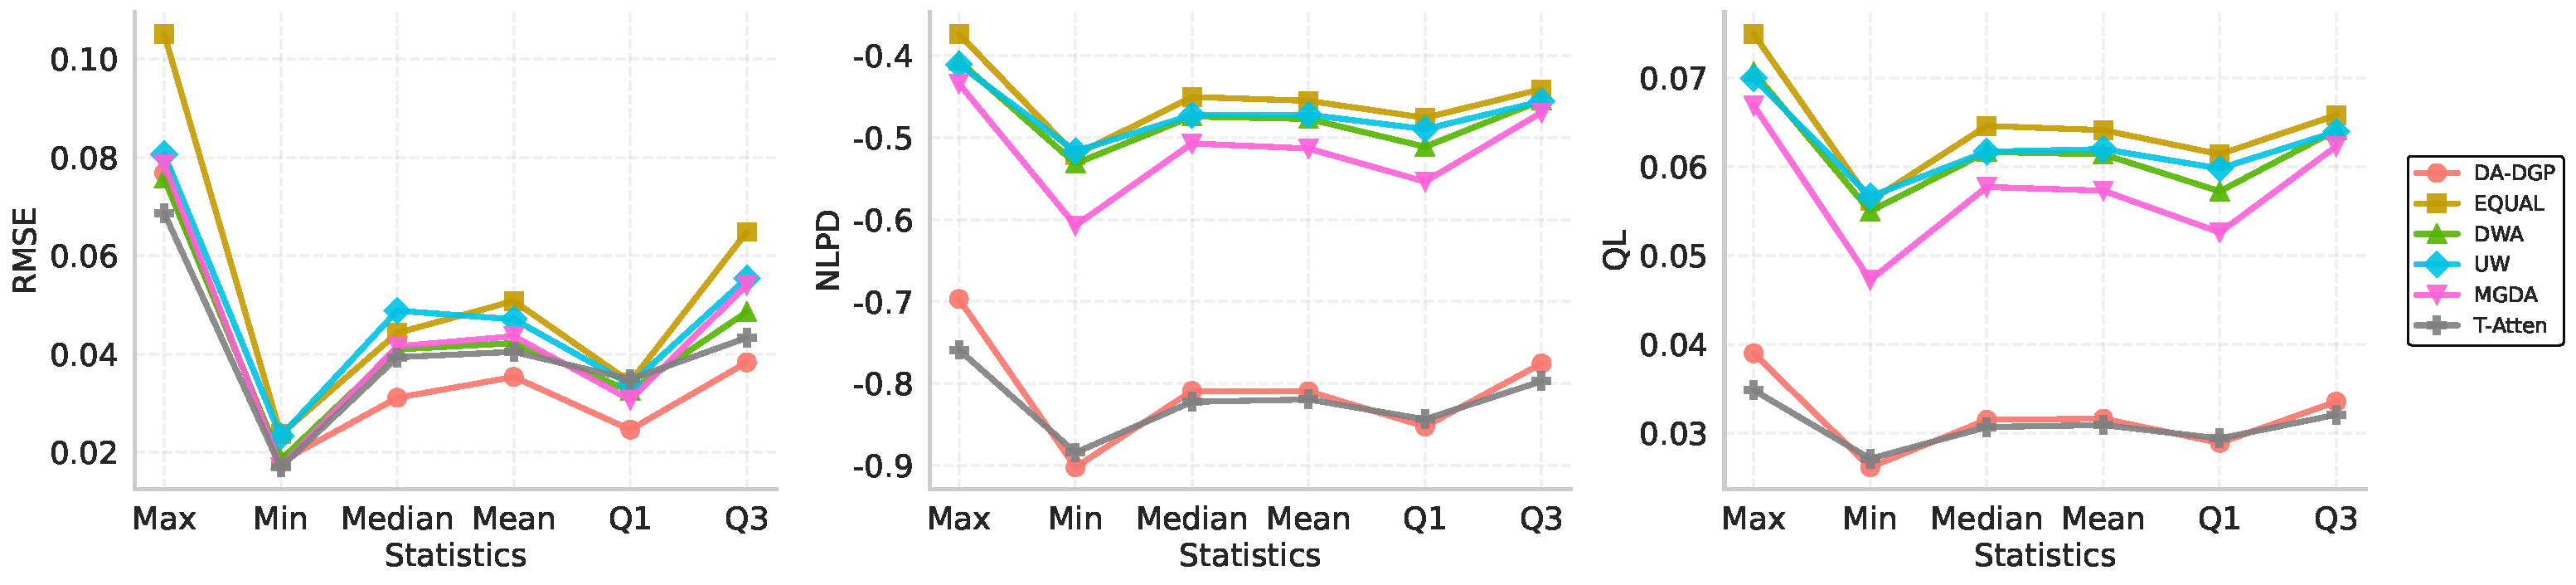
\includegraphics[width=0.8\textwidth]{FIG4a.pdf}
				\caption{Task 1 ($y_1$)}
				\label{fig:task1_curves}
			\end{subfigure}
		
	%	\vspace{0.4cm} % 增加行间距，防止图挨得太近
		
		% --- 第二行: Task 2 (b) ---
		\begin{subfigure}[b]{1.0\textwidth}
				\centering
				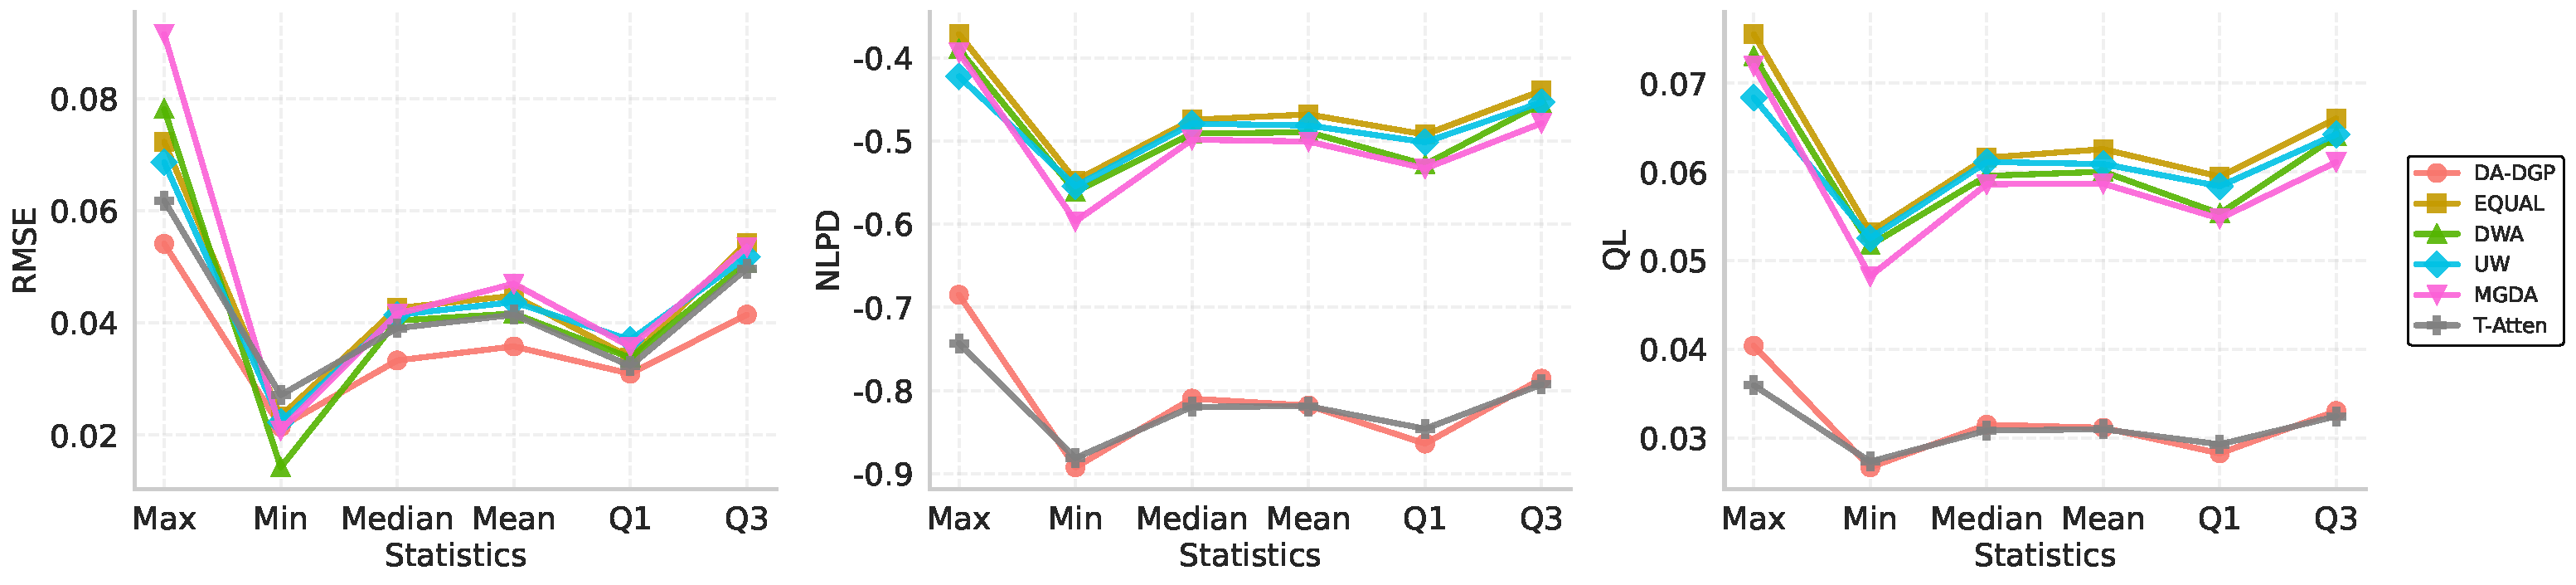
\includegraphics[width=0.8\textwidth]{FIG4b.pdf}
				\caption{Task 2 ($y_2$)}
				\label{fig:task2_curves}
			\end{subfigure}
		
	%	\vspace{0.4cm} % 增加行间距
		
		% --- 第三行: Task 3 (c) ---
		\begin{subfigure}[b]{1.0\textwidth}
				\centering
				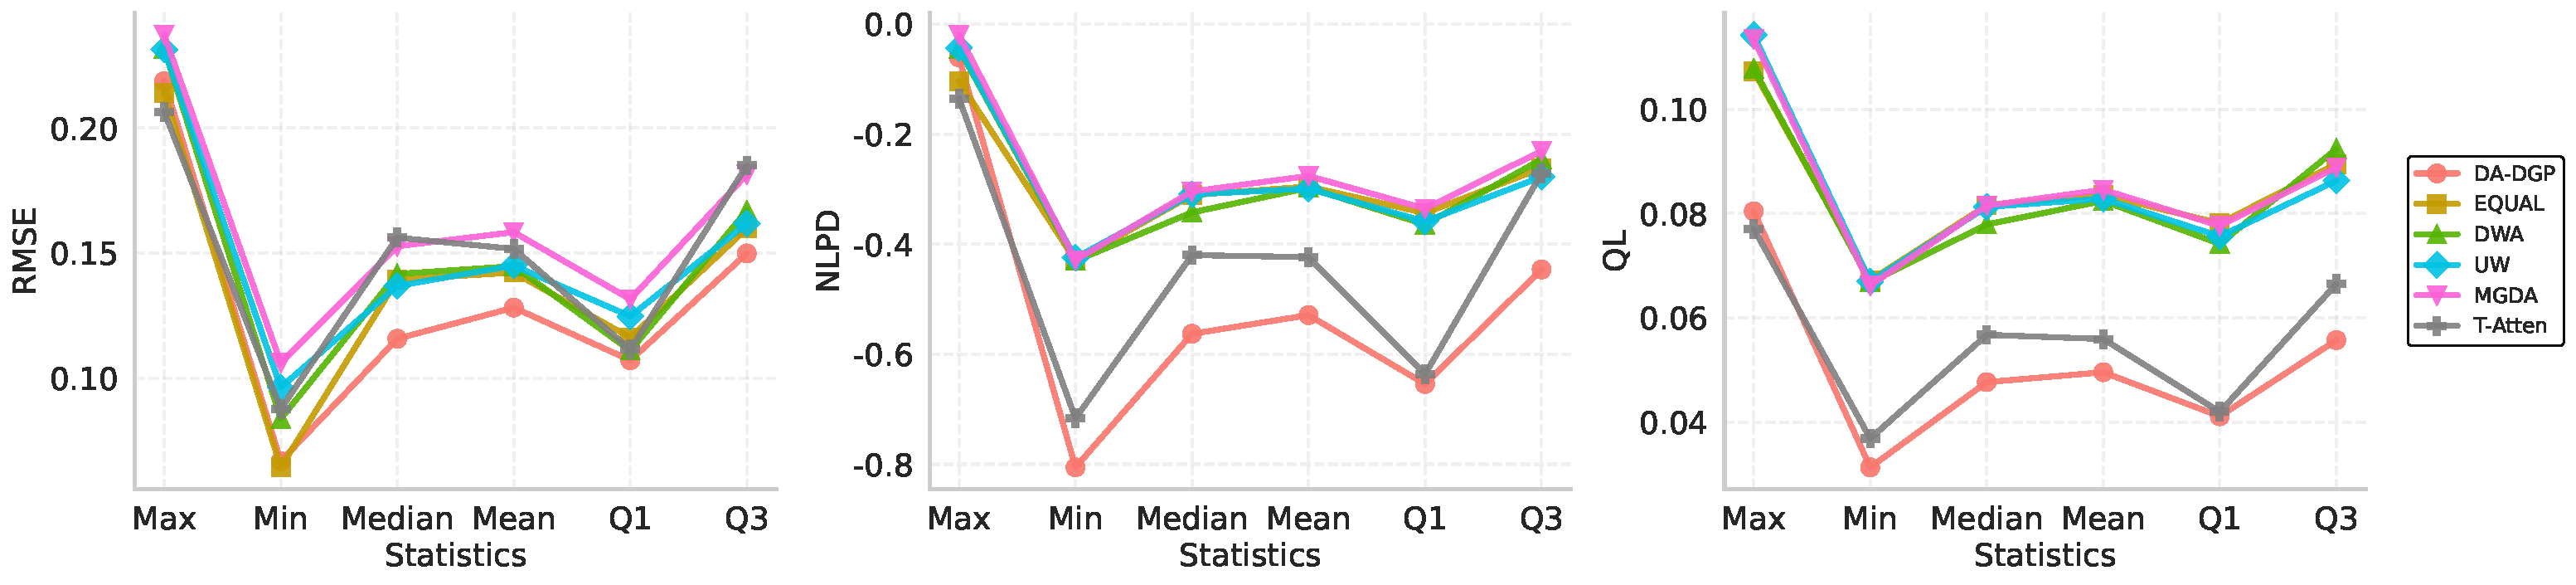
\includegraphics[width=0.8\textwidth]{FIG4c.pdf}
				\caption{Task 3 ($y_3$)}
				\label{fig:task3_curves}
			\end{subfigure}
		
		\caption{Performance metric curves for the three tasks.}
		\label{fig:performance_curves}
	\end{figure}

	
	
	\newpage
\begin{thebibliography}{99}
	
	% 注意：\bibitem 后面的 [Titsias(2009)] 是必须的，natbib 靠它来生成 (Author, Year)
	\bibitem[Titsias(2009)]{titsias2009variational}
	Titsias, M. (2009). 
	Variational Learning of Inducing Variables in Sparse Gaussian Processes. 
	\textit{Artificial Intelligence and Statistics (AISTATS), PMLR}, 5, 567--574.
	
	% 注意：\bibitem 后面的 [Knoblauch et~al.(2019)] 是必须的
	\bibitem[Knoblauch et~al.(2019)]{knoblauch2019generalized}
	Knoblauch, J., Jewson, J., \& Damoulas, T. (2019). 
	Generalized Variational Inference: Three arguments for deriving new Posteriors. 
	\textit{arXiv preprint arXiv:1904.02063}.
	
\end{thebibliography}
	
	
	
	
	
	
	
	
	
	
	
	
	
	
	
	
	
	
	
	
	
	
	
	
	
\end{document}